%************************************************
\chapter{Results}\label{ch:Results}
%************************************************

In this section we explore the result of this works.

We mentioned 4 metrics that we were considering for this work:

\begin{itemize}
\item Minimize the amount of space required
\item Minimize the start up time of containers
\item Limit the number of files in each CVMFS catalogs
\item Minimize the complexity of managing the filesystem itself
\end{itemize}

All the measurement are going to be done against a CVMFS repository containing
images necessary for standard HEP work.

In order to quantify the amount of space required we are simply going to
measure the amount of space that the repository uses, we will compare this
figure with the amount of data that the repository provides and with a simple
summation over the size of the layers stored in the repository.

The startup time of a container is greatly influenced by the cache layer in all
cases, either if we serve the content with CVMFS or if the content is already
cached in the hosting machine.

We will measure the startup time of all kind of technologies with and without
cache a significant number of times, the measurement are made inside the CERN
data center where we assume a stable and reliable internet connection.

The amount of files in each CVMFS catalog is a simple measurement, since the
amount of catalogs is rather big we will synthetize this measurement.

To measure the complexity of managing the filesystem we are going to measure
the cyclomatic complexity of the software that we use to manage it.

\section{Space Requirement}

By default CVMFS stores all its content in \texttt{/srv}, hence the most
reliable way to obtain the size of the repository is to analyze the storage
used under \texttt{/srv}. The storage required for the whole repository is of
~27G calculate with the \texttt{df} unix utility as show in
\ref{lst:data-storage}.

\begin{minipage}{\linewidth}
\begin{lstlisting}[language=bash,caption={Storage require to store the whole repository},label={lst:data-storage}]
>> df -h /srv
Filesystem      Size  Used Avail Use% Mounted on
/dev/vdb        197G   27G  161G  15% /srv # <-- I believe is too much, most likely an error
\end{lstlisting}
\end{minipage}

We than obtain the size of the two hidden folder \textit{.layers} and
\textit{.flat} using the `cvmfs\_server list-catalogs` command which provides us
with the number of files in each catalog and the number of bytes that each
catalog manage.

\begin{table}[]
\begin{tabular}{|l|ll|}
\hline
     & .flat & .layers \\ \hline
Size & 28    & 27      \\ \hline
\end{tabular}
\caption{Apparent size in GB of the two folder \textit{.layers} and \textit{.flat}}
\label{tab:size-of-repo}
\end{table}

We can see that the Content-Addressable-Storage used by CVMFS helps a lot by
reducing the amount of space required to host the repository by half, which
make sense since the \textit{.layers} and the \textit{.flat} contains the exact
same files.

\section{Container Startup Time}

This Section explores the startup time of the containers host in the CVMFS
file-system.

We will show the average time of starting a container, start the python shell
inside the container and executing the exit command inside the shell.

We decide for this simulation because it requires to have access to  the python
interpreter in the container, which is a executable of not negligible size.

We propose 8 scenarios that we synthesize in the Table \ref{tab:benchmark}
below.


% Please add the following required packages to your document preamble:
% \usepackage{multirow}
\begin{table}[]
\begin{tabular}{|l|l|l|l|l|l|}
\hline
\multicolumn{2}{|l|}{\multirow{2}{*}{}}            & \multicolumn{2}{l|}{Cache} & \multicolumn{2}{l|}{No Cache} \\ \cline{3-6} 
\multicolumn{2}{|l|}{}                             & Avg          & STD         & Avg            & STD          \\ \hline \hline
\multirow{2}{*}{Thin-Image on CVMFS} & Singularity & 10.31        & 4.38        & 29.13          & 4.02         \\ \cline{2-6} 
                                     & Docker      & 96.74        & 5.40        & 180.02         & 35.13        \\ \hline \hline
\multirow{2}{*}{Naive}               & Singularity & 7.38         & 2.07        & 1884.76        & 366.84       \\ \cline{2-6} 
                                     & Docker      & 95.26        & 5.29        & 1279.21        & 168.99       \\ \hline
\end{tabular}
\caption{Benchmark of startup time of a containers, the first number is the average while the second is the standard deviation. The units are in hundredths of seconds. $n = 100$}
\label{tab:benchmark}
\end{table}

We ran the benchmark 100 times, and we collect the startup time with the unix
utility \texttt{time}. The code that we used to obtain the number is available
on the listing on Section \ref{sec:benchmark-code}

We can see that the use of CVMFS is a huge help when the cache is not
available, moreover its overhead is almost negligiable when the cache is
present. Is interesting to know that the containers hosted in CVMFS without
cache starts in an amount of time comparable to the containers hosted naively
but using cache (4 times slower in the case of Singularity and 2 times slower
in the case of Docker.)

\section{File in the sub-catalogs}

CVMFS provides a rule of thumb about the number of files that should be hosted
in each catalog to avoid stressing the sub-catalog too much. It suggest to
limit the amount of file to less than 200000.

Using again the CVMFS command `cvmfs\_server list-catalogs` we obtain the
number of files in each catalog.

We show the result in the graphs \ref{fig:layercatalog}, \ref{fig:flatcatalog},
\ref{fig:loglayercatalog} and \ref{fig:logflatcatalog}.

We can see how all the catalogs have less than 200000 entries respecting the
suggestion of CVMFS.

Moreover, we can notice how the amount of file in a Docker image follows a
power distribution.

\begin{figure}[]{}
    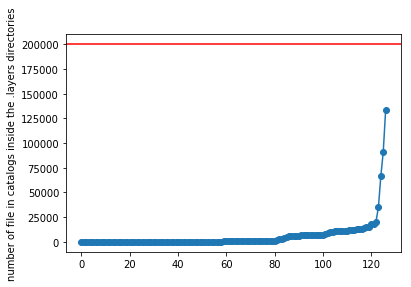
\includegraphics[]{gfx/catalogs-layer}
        \caption{Number of files inside the catalogs in the \textit{.layer} directory.}
        \label{fig:layercatalog}
\end{figure}

\begin{figure}[]{}
    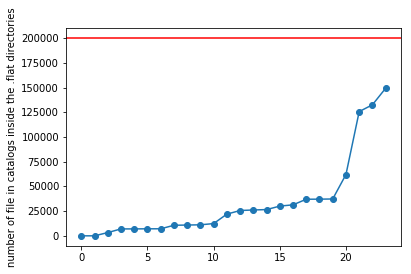
\includegraphics[]{gfx/catalogs-flat}
        \caption{Number of files inside the catalogs in the \textit{.flat} directory.}
        \label{fig:flatcatalog}
\end{figure}

\begin{figure}[]{}
    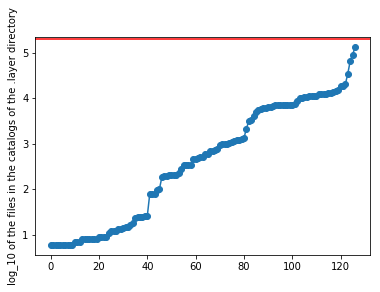
\includegraphics[]{gfx/catalogs-layer-log}
        \caption{Logarithm of the number of files inside the catalogs in the \textit{.layer} directory.}
        \label{fig:loglayercatalog}
\end{figure}

\begin{figure}[]{}
    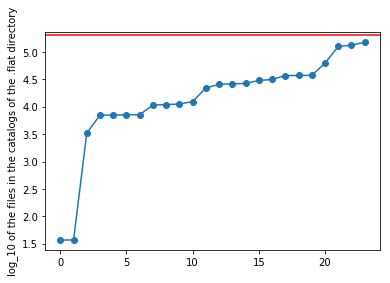
\includegraphics[]{gfx/catalogs-flat-log}
        \caption{Logarithm of the number of files inside the catalogs in the \textit{.flat} directory.}
        \label{fig:logflatcatalog}
\end{figure}

\section{Complexity}

In order to estimate the complexity of managing the file-system we decide to
use the cyclomatic complexity of he tool that create and manage the file-system
itself that we discuss on Chapter \ref{ch:implementation}. We used
\textit{gocylo} \cite{gocylo} a command line tool that calculate the cyclomatic
complexity of functions written in the Go(lang) languange.

\begin{lstlisting}[language=bash,
    caption={Result of the cyclomatic complexity analysis, only function with complexity greater or equal to 3 are shown},label={lst:cyclomatic}]
>> gocyclo main.go cmd/ lib/ docker-api/
37 lib ConvertWish lib/conversion.go:33:1
15 lib ParseImage lib/parse.go:9:1
14 lib AddManifestToRemoveScheduler lib/cvmfs.go:299:1
12 lib GarbageCollectSingleLayer lib/garbage_collection.go:62:1
12 lib (Image).GetChanges lib/image.go:145:1
12 lib (Image).downloadLayer lib/image.go:436:1
11 lib SaveLayersBacklink lib/cvmfs.go:219:1
11 lib IngestIntoCVMFS lib/cvmfs.go:23:1
9 lib requestAuthToken lib/image.go:519:1
9 lib CreateSymlinkIntoCVMFS lib/cvmfs.go:99:1
9 lib RemoveDirectory lib/cvmfs.go:426:1
8 lib (Image).GetLayers lib/image.go:375:1
7 lib FindImageToGarbageCollect lib/garbage_collection.go:15:1
7 lib (Image).GetReference lib/image.go:70:1
6 lib AlreadyConverted lib/conversion.go:317:1
6 lib getBacklinkFromLayer lib/cvmfs.go:176:1
6 lib (*execCmd).Start lib/exec_commands.go:35:1
5 lib getManifestWithUsernameAndPassword lib/image.go:303:1
5 lib (Image).GetManifest lib/image.go:125:1
5 lib ParseYamlRecipeV1 lib/recipe.go:23:1
5 lib firstRequestForAuth lib/image.go:337:1
4 lib (Singularity).IngestIntoCVMFS lib/image.go:262:1
4 lib parseBearerToken lib/image.go:499:1
4 lib (Image).PrintImage lib/image.go:93:1
4 lib (Image).DownloadSingularityDirectory lib/image.go:238:1
3 dockerutil MakeThinImage docker-api/util.go:47:1
3 lib (Image).GetSimpleReference lib/image.go:83:1
3 lib (Image).WholeName lib/image.go:49:1
3 lib CreateWish lib/wish.go:26:1
3 lib ExecCommand lib/exec_commands.go:18:1
\end{lstlisting}

While the cyclomatic complexity is very high is important to note that
idiomatic golang codes requires to manually check every possible error returned
by other functions, all these checks increase dramatically the cyclomatic
complexity of the code. Indeed there are 19 error check without any logic in
the code but simply returning early in the ConvertWish function.


\section{Code to get the numbers}\label{sec:benchmark-code}


\begin{lstlisting}[language=bash,
    caption={Script used to capture the startup time of singularity with image hostes in CVMFS using CVMFS cache}]
#!/bin/bash

for i in {1..101}; 
do 
    /usr/bin/time -f "%U,%S,%E" \
        singularity exec \
            /cvmfs/thin.osg.cern.ch/library/python:latest \
            python -c "quit()"; 
done
\end{lstlisting}


\begin{lstlisting}[language=bash,
    caption={Script used to capture the startup time of singularity with image hostes in CVMFS without cache}]
#!/bin/bash

for i in {1..101}; 
do 
    #cleanup the cvmfs cache
    cvmfs_config wipecache >> /dev/null; 
    
    /usr/bin/time -f "%U,%S,%E" \
        singularity exec \
            /cvmfs/thin.osg.cern.ch/library/python:latest \
            python -c "quit()"; 
done
\end{lstlisting}


\begin{lstlisting}[language=bash,
    caption={Script used to capture the startup time of docker thin-images using both CVMFS and Docker cache}]
#!/bin/bash

docker pull thin-python:latest

for i in {1..101}; 
do 
    /usr/bin/time -f "%U,%S,%E" \
        docker run thin-python:latest python -c "quit()"; 
done
\end{lstlisting}



\begin{lstlisting}[language=bash,
    caption={Script used to capture the startup time of docker thin-images without Docker nor CVMFS cache}]
#!/bin/bash

for i in {1..101}; 
do 
    #cleanup the cvmfs cache
    cvmfs_config wipecache >> /dev/null; 
    
    # remove the layers from the docker cache
    docker rmi thin-python:latest -f >> /dev/null; 
    
    # cleanup any remaining data from the system
    docker system prune -a -f; 

    /usr/bin/time -f "%U,%S,%E" \
        docker run thin-python:latest python -c "quit()"; 
done
\end{lstlisting}




\begin{lstlisting}[language=bash,
caption={Script used to capture the startup time of Docker standard images without Docker cache}]
#!/bin/bash

for i in {1..101}; 
do 
    # remove the local image of python
    docker rmi -f python:latest; 

    # cleanup any remaining data from the system
    docker system prune -a -f; 
    
    /usr/bin/time -f "%S,%U,%E" \
        -o ~/start-time-docker-standard-no-cache.csv -a \
        docker run python:latest python -c "quit()"; 
done
\end{lstlisting}


\begin{lstlisting}[language=bash,
    caption={Script used to capture the startup time of Singularity running Docker standard images without Singularity cache}]
#!/bin/bash

for i in {1..101}; 
do
    # cleanup the singularity cache directory
    rm -rf /root/.singularity/docker; 
    
    /usr/bin/time -f "%S,%U,%E" \
        -o ~/start-time-singularity-standard-no-cache.csv -a \
        singularity exec docker://python:latest \
            python -c "quit()"; 
done
\end{lstlisting}



\begin{lstlisting}[language=bash,
    caption={Script used to capture the startup time of Singularity running images unpacked on the local file-system, hence with cache}]
#!/bin/bash

for i in {1..101}; 
do 
    /usr/bin/time -f "%S,%U,%E" \
        -o ~/start-time-singularity-standard.csv -a \
        singularity exec python_latest/ python -c "quit()"; 
done

\end{lstlisting}

\begin{lstlisting}[language=bash,caption={Script used to capture the startup time of docker thin-images without cache}]
#!/bin/bash
for i in {1..101}; 
do 
    # clean the CVMFS cache
    cvmfs_config wipecache >> /dev/null; 
        
    # clean the docker cache
    docker rmi thin-osg/library/python:latest -f >> /dev/null; 
        
    # run and measure the start up time
    /usr/bin/time -f "%S,%U,%E" \
        -o ~/start-time-docker-no-cache.csv -a \ 
        docker run thin-osg/library/python:latest \
            python -c "quit()"; 
done
\end{lstlisting}
